\documentclass[review]{elsarticle}

\usepackage{amsmath}
\usepackage{dirtytalk}
\usepackage{subcaption}
\usepackage[usenames]{xcolor}
\usepackage{lineno,hyperref}
\modulolinenumbers[5]

\journal{Composites Part A}

%%%%%%%%%%%%%%%%%%%%%%%
%% Elsevier bibliography styles
%%%%%%%%%%%%%%%%%%%%%%%
%% To change the style, put a % in front of the second line of the current style and
%% remove the % from the second line of the style you would like to use.
%%%%%%%%%%%%%%%%%%%%%%%

%% Numbered
%\bibliographystyle{model1-num-names}

%% Numbered without titles
%\bibliographystyle{model1a-num-names}

%% Harvard
%\bibliographystyle{model2-names.bst}\biboptions{authoryear}

%% Vancouver numbered
%\usepackage{numcompress}\bibliographystyle{model3-num-names}

%% Vancouver name/year
%\usepackage{numcompress}\bibliographystyle{model4-names}\biboptions{authoryear}

%% APA style
%\bibliographystyle{model5-names}\biboptions{authoryear}

%% AMA style
%\usepackage{numcompress}\bibliographystyle{model6-num-names}

%% `Elsevier LaTeX' style
\bibliographystyle{elsarticle-num}
%%%%%%%%%%%%%%%%%%%%%%%

\begin{document}

\begin{frontmatter}

\title{Energy release rate of the fiber/matrix interface crack in cross-ply $\left[0_{2kn}^{\circ},90_{n}^{\circ}\right]_{S}$ laminates under transverse loading: debond/bi-material interface interaction}
%\tnotetext[mytitlenote]{Fully documented templates are available in the elsarticle package on \href{http://www.ctan.org/tex-archive/macros/latex/contrib/elsarticle}{CTAN}.}

%% Group authors per affiliation:
%\author{Luca Di Stasio\fnref{myfootnote}}
%\address{Radarweg 29, Amsterdam}
%\fntext[myfootnote]{Since 1880.}

%% or include affiliations in footnotes:
\author[nancy,lulea]{Luca Di Stasio}
\author[lulea]{Janis Varna}
\author[nancy]{Zoubir Ayadi}
%\ead[url]{www.elsevier.com}

%\author[mysecondaryaddress]{Global Customer Service\corref{mycorrespondingauthor}}
%\cortext[mycorrespondingauthor]{Corresponding author}
%\ead{support@elsevier.com}

\address[nancy]{Universit\'e de Lorraine, EEIGM, IJL, 6 Rue Bastien Lepage, F-54010 Nancy, France}
\address[lulea]{Lule\aa\ University of Technology, University Campus, SE-97187 Lule\aa, Sweden}

\begin{abstract}
\noindent
%\textcolor{purple}{{\em Priority}: 1}\\
%\textcolor{purple}{{\em Target journal(s)}: Composites Part B: Engineering, Composites Part A: Applied Science and Manufacturing, Composite Structures, Journal of Composite Materials, Composite Communications}\\
The effects of crack shielding, fiber content and ratio of $0^{\circ}$ to $90^{\circ}$ ply thickness on fiber/matrix debond growth in thin cross-ply laminates are investigated with Representative Volume Elements (RVEs) of different ordered microstructures. Debond growth is characterized by the estimation of the Energy Release Rates (ERRs) using the Virtual Crack Closure Technique (VCCT) and the J-integral. It is found that 
\end{abstract}

\begin{keyword}
Polymer-matrix Composites (PMCs)\sep Thin-ply\sep Transverse Failure \sep Debonding \sep Finite Element Analysis (FEA)
\end{keyword}


\end{frontmatter}

\linenumbers

%%%%%%%%%%%%%%%%%%%%%%%%%%%%%%%%%%%%%%%%%%%%%%%%%%%%%%%%%%%%%%%%%%%
% 1. INTRODUCTION
%%%%%%%%%%%%%%%%%%%%%%%%%%%%%%%%%%%%%%%%%%%%%%%%%%%%%%%%%%%%%%%%%%%

\section{Introduction}

Since the development of the \emph{spred tow} technology or \say{FUKUI method}~\cite{Kawabe2008,Kawabe2008en}, significant efforts have been directed toward the characterization of \emph{thin-ply} laminates~\cite{Sasayama2003,Yamaguchi2005,Tsai2005,Sihn2007,Yokozeki2008,Yokozeki2010,Saito2012,Arteiro2013,Arteiro2014,Amacher2014,Guillamet2014,Huang2018,Cugnoni2018} and their application to mission-critical structures in the aerospace sector~\cite{Moon2011,Kim2017,Kopp2017,McCarville2018}.\\
At the lamina level, the use of \emph{thin-plies} leads to more regular and homogeneous microstructures but no significant imporvement in static properties except for an apparent improvement in compressive strength~\cite{Amacher2014}. Improvements in fatigue life have been observed, although contrasting results can be found in the literature~\cite{Yamaguchi2005,Tsai2005,Sihn2007}. The beneficial effect of the use of \emph{thin-plies} with respect to damage propagation has been instead commonly observed by different researchers under static~\cite{Sasayama2003,Sihn2007,Yokozeki2008,Yokozeki2010,Saito2012,Arteiro2013,Arteiro2014,Amacher2014}, fatigue~\cite{Yamaguchi2005,Sihn2007,Yokozeki2008,Yokozeki2010,Amacher2014} and impact loadings~\cite{Sihn2007,Yokozeki2008,Yokozeki2010,Amacher2014}. It seems apparent that \emph{thin-ply} laminates possess an increased ability to delay, and in some cases even suppress, the onset and propagation of transverse cracks (or matrix or micro-cracks).\\
The first appearance of transverse cracking phenomena is known to be characterized by the appearance of fiber/matrix interface cracks (also referred to as debonds), which grow along the fiber's arc direction, then kink out of the interface and coalesce forming a transverse crack~\cite{Bailey1981}. Different approaches have been applied to model the initiation and growth of debonds. The Cohesive Zone Model (CZM) has been used to mimic the propagation of debonds along fiber interfaces; coupled with a failure criterion for the matrix, it has provided simulations of the growth of transverse cracks starting from a virgin material~\cite{Kushch2011,Canal2012,Bouhala2013,Herraez2015}. The main advantages of this approach are the possibility to observe the development of a simulated crack path and to record a load-displacement curve to compare with experimental measurement. However, various observations cast a doubt about the applicability of the CZM: the bi- (for 2D models) and tri- (in 3D) axiality of the matrix stress state in the inter-fiber region that is linked with a cavitation-like failure of the polymer~\cite{Asp1995}; the locality and mode dependency of the interface failure~\cite{Mantic2009}; the problematic use at the microscopic level of properties measured in UD specimens at the laminate level~\cite{Canal2012}. A second approach that obviates these drawbacks is the application of Linear Elastic Fracture Mechanics (LEFM) arguments to the study of debond growth. The analysis focuses on the evaluation of Mode I and Mode II Energy Release Rate (ERR) at the crack tip by means of the Virtual Crack Closure Technique (VCCT)~\cite{Krueger2004} or the J-Integral method~\cite{Rice1968}. The stress and strain field, required for the ERR computation, can be solved by application of different methodologies such as analytical solutions~\cite{Toya1974}, the Boundary Element Method (BEM)~\cite{Paris1996} or the Finite Element Method (FEM)~\cite{Zhuang2018}. Different works have followed this approach and studied models of one or two fibers in an effectively infinite matrix~\cite{Correa2011,Correa2013,Correa2014,Sandino2016,Sandino2018} and of an hexagonal cluster of fibers in an effectively infinite homogenized UD composite~\cite{Varna2017,Zhuang2018}. The problem of debond growth along the fiber-matrix interface in a cross-ply laminate has been only addressed very recently in~\cite{Velasco2018,Paris2018}, where the author embed a single partially debonded fiber in an effectively infinite homogenized $90^{\circ}$ ply bounded by homogenized $0^{\circ}$ layers. Thus, the effect of debond-debond interaction and of the relative proximity of a bi-material interface on the debond's ERR in cross-ply laminates is yet to be addressed. The present work is devoted to this problem. Models of Repeating Unit Cells (RUCs) are developed to represent laminates with different degrees of damage (here only in the form of debonds). The number of fully bonded fibers across the thickness of the $90^{\circ}$ ply is varied in order to investigate the effect of the proximity of the bi-material interface. The thickness of the bounding $0^{\circ}$ layers is also analyzed as a parameter of the study. The stress and strain fields are solved with the Finite Element Method in Abaqus~\cite{abq12} and the crack characterized by its Mode I and Mode II ERR, calculated with the VCCT and the J-integral method.

%%%%%%%%%%%%%%%%%%%%%%%%%%%%%%%%%%%%%%%%%%%%%%%%%%%%%%%%%%%%%%%%%%%
% 2. RVE MODELS AND FE DISCRETIZATION
%%%%%%%%%%%%%%%%%%%%%%%%%%%%%%%%%%%%%%%%%%%%%%%%%%%%%%%%%%%%%%%%%%%

\section{RVE models \& FE discretization}

% 2.1 Introduction and nomenclature

\subsection{Introduction \& Nomenclature}\label{subsec:names}

\subsection{Models of Representative Volume Element (RVE)}\label{subsec:rve}

\begin{figure}[!h]
\centering
  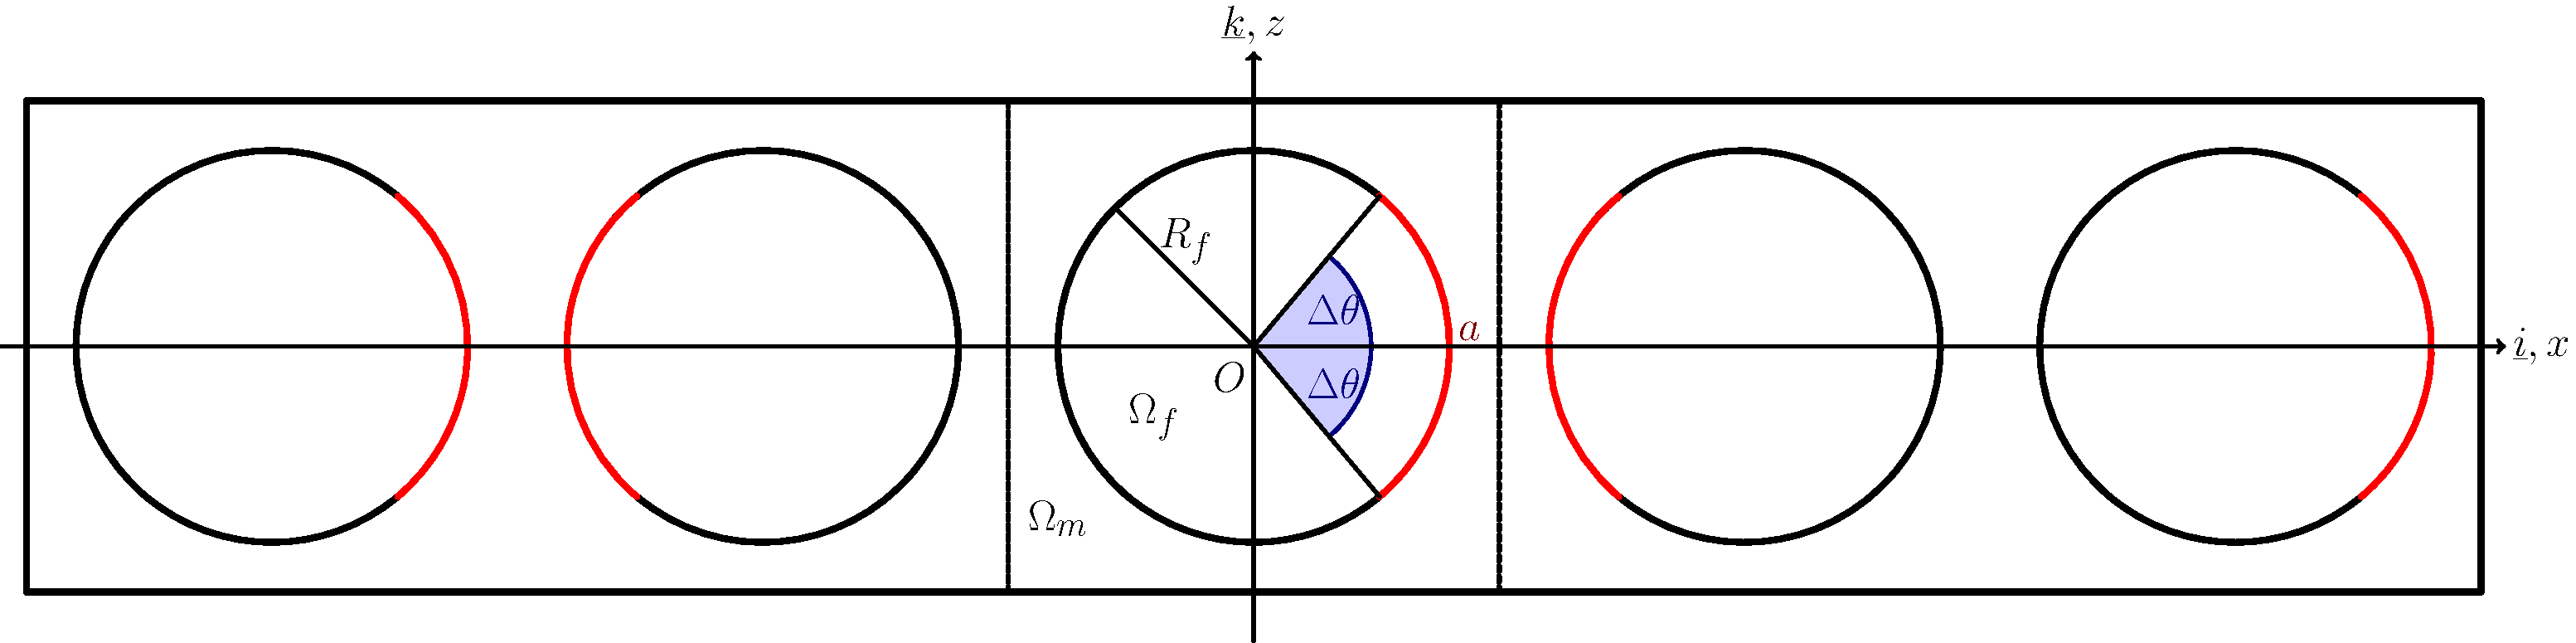
\includegraphics[width=\textwidth]{freeThinPly.pdf}
\caption{Models of ultra-thin UD composites with a single ``row'' of fibers and debonds repeating at different distances.}\label{fig:laminateModelsA}
\end{figure}

\begin{figure}[!h]
\centering
        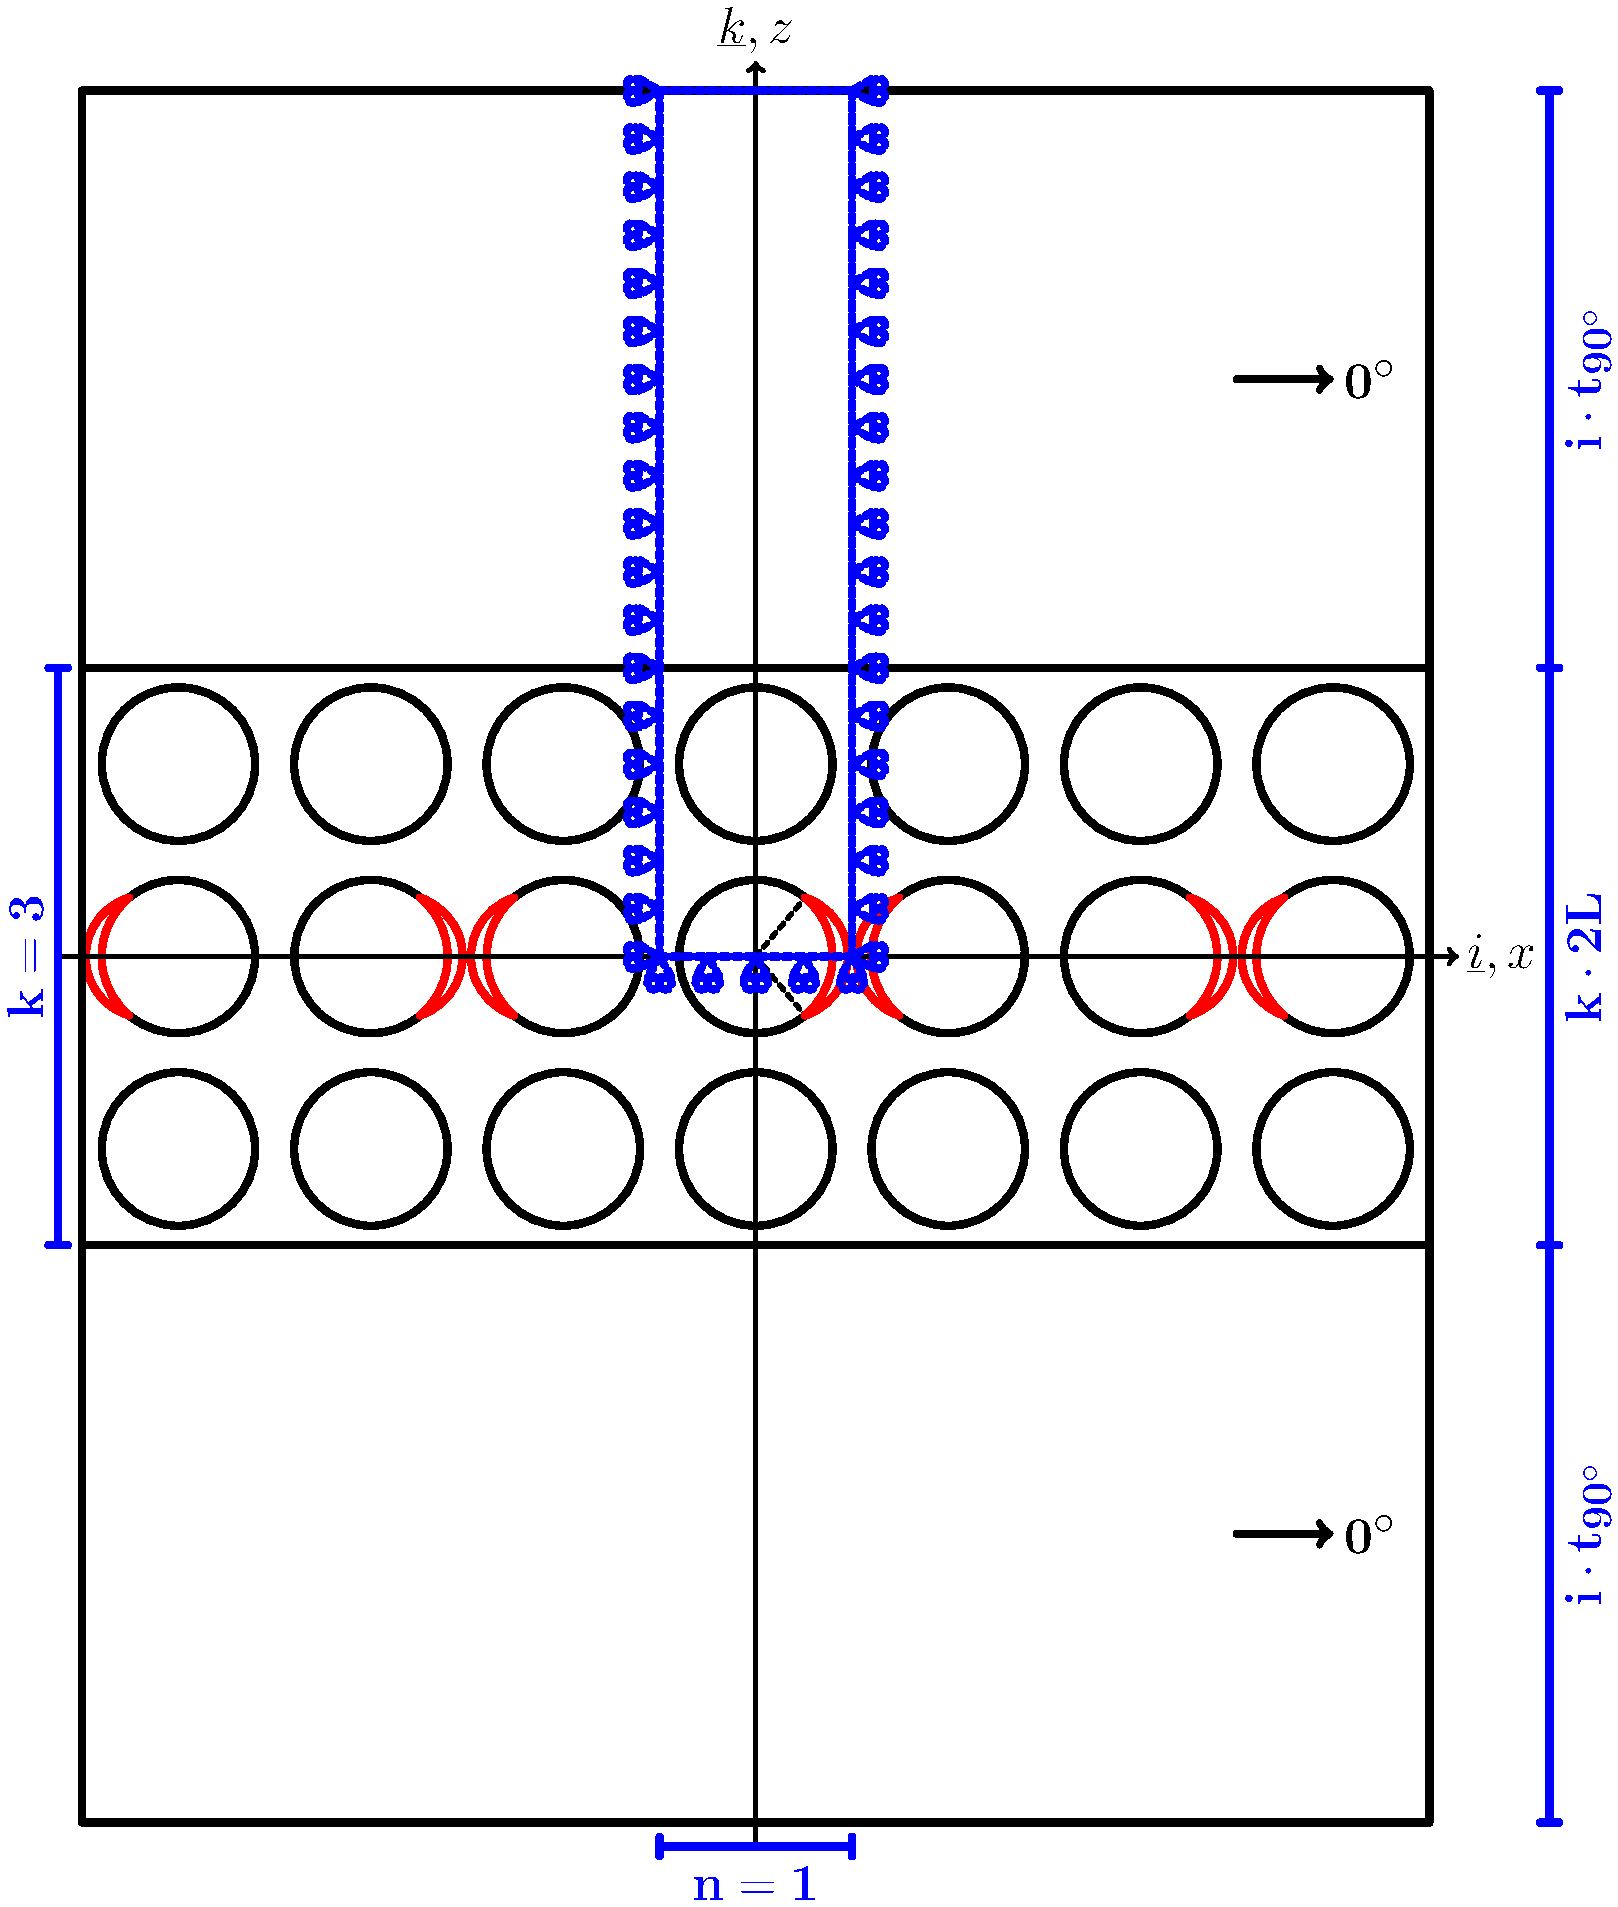
\includegraphics[height=0.3\textheight]{thickPlycentraldebondsline.pdf}
  %      \caption{Multiple rows of fibers with debonds appearing on each fiber beloging to the central row: model $1\times k-free$ ($k=3$ in the figure).}\label{subfig:thickplycentraldebonds}
\caption{Models of UD composites with different ``rows'' of fibers and debonds repeating at different distances.}\label{fig:laminateModelsB}
\end{figure}

\begin{figure}[!h]
\centering
        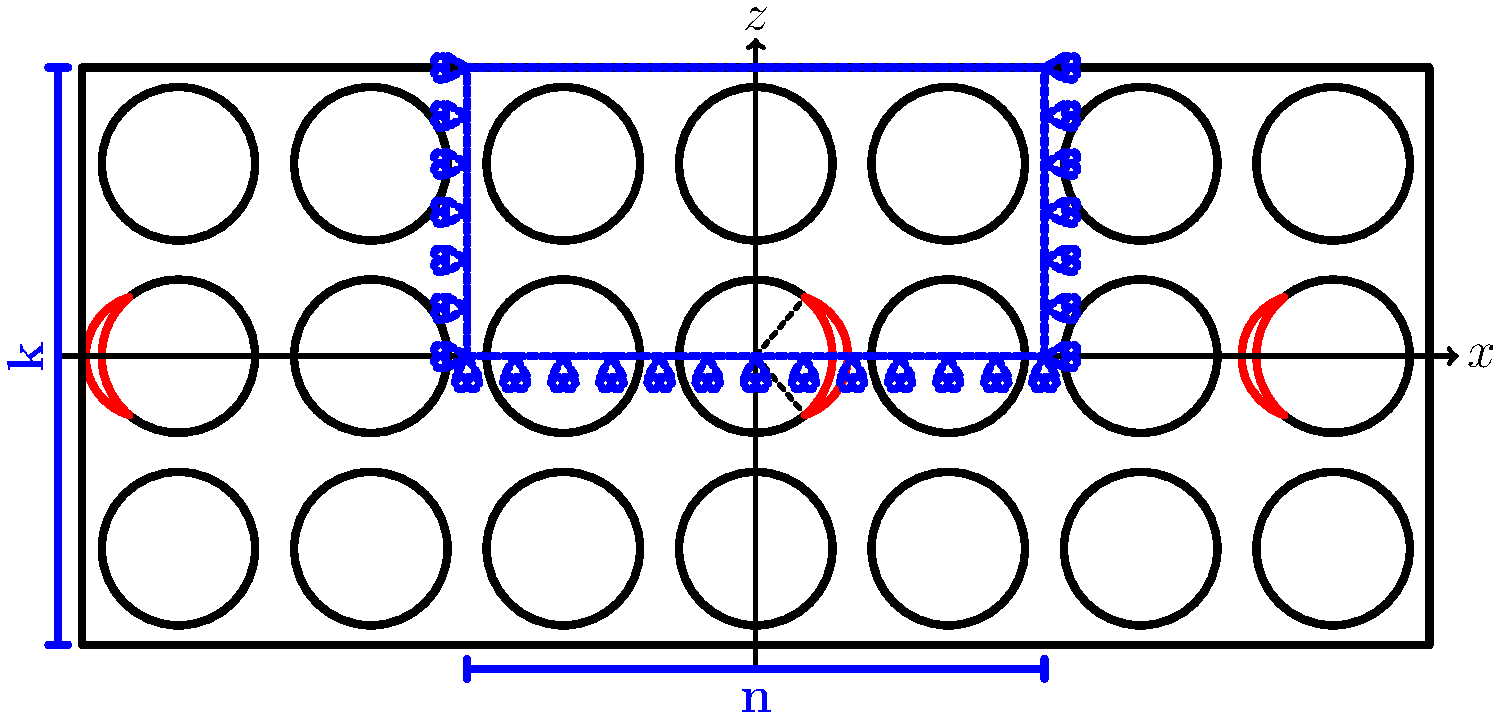
\includegraphics[width=\textwidth]{thickPly.pdf}
   %    \caption{Mutiple rows of fibers with a debond appearing every $n$ fibers within the central row: model $n\times k-free$ ($n=3$ and $k=3$ in the figure).}\label{subfig:thickply}
\caption{Models of UD composites with different ``rows'' of fibers and debonds repeating at different distances.}\label{fig:laminateModelsB}
\end{figure}

\subsection{Finite Element (FE) discretization}



\section{Results \& Discussion}

\subsection{Effect of Fiber Volume Fraction}

\textcolor{blue}{The effect is similar for all the different BC cases, it's enough to show some of them to exemplify. $G_{I}$ in Fig.~\ref{fig:volumefractionMI}, $G_{II}$ in Fig.~\ref{fig:volumefractionMII}.}

\textcolor{purple}{Graphics of ERR vs $\Delta\theta$, one curve for each $V_{f}$, one graphic for each selected BC. Selected BC: free, coupling, some examples with fibers (see captions).}

\begin{figure}[!h]
\centering
    \begin{subfigure}[b]{0.45\textwidth}
        %\includegraphics[width=\textwidth]{}
        \caption{Single fiber model with free boundary on top.}\label{subfig:volfracfreeMI}
    \end{subfigure} ~
    \begin{subfigure}[b]{0.45\textwidth}
        %\includegraphics[width=\textwidth]{}
        \caption{Single fiber model with coupling of vertical displacements along the upper boundary.}\label{subfig:volfraccouplingMI}
    \end{subfigure}

    \begin{subfigure}[b]{0.45\textwidth}
        %\includegraphics[width=\textwidth]{}
        \caption{1 fiber each side.}\label{subfig:volfrac1eachsideMI}
    \end{subfigure} ~
    \begin{subfigure}[b]{0.45\textwidth}
        %\includegraphics[width=\textwidth]{}
        \caption{1 fiber above.}\label{subfig:volfrac1aboveMI}
    \end{subfigure}

    \begin{subfigure}[b]{0.45\textwidth}
        %\includegraphics[width=\textwidth]{}
        \caption{5 fibers each side.}\label{subfig:volfrac5eachsideMI}
    \end{subfigure} ~
    \begin{subfigure}[b]{0.45\textwidth}
        %\includegraphics[width=\textwidth]{}
        \caption{5 fibers above.}\label{subfig:volfrac5aboveMI}
    \end{subfigure}

    \begin{subfigure}[b]{0.45\textwidth}
        %\includegraphics[width=\textwidth]{}
        \caption{10 fibers each side.}\label{subfig:volfrac10eachsideMI}
    \end{subfigure} ~
    \begin{subfigure}[b]{0.45\textwidth}
        %\includegraphics[width=\textwidth]{}
        \caption{10 fibers above.}\label{subfig:volfrac10aboveMI}
    \end{subfigure}

    \begin{subfigure}[b]{0.45\textwidth}
        %\includegraphics[width=\textwidth]{}
        \caption{1 fiber each side, 1 above.}\label{subfig:volfrac1eachside1aboveMI}
    \end{subfigure} ~
    \begin{subfigure}[b]{0.45\textwidth}
        %\includegraphics[width=\textwidth]{}
        \caption{3 fibers each side, 1 above.}\label{subfig:volfrac3eachside1aboveMI}
    \end{subfigure}

    \begin{subfigure}[b]{0.45\textwidth}
        %\includegraphics[width=\textwidth]{}
        \caption{2 fibers each side, 2 above.}\label{subfig:volfrac2eachside2aboveMI}
    \end{subfigure} ~
    \begin{subfigure}[b]{0.45\textwidth}
        %\includegraphics[width=\textwidth]{}
        \caption{5 fibers each side, 2 above.}\label{subfig:volfrac5eachside2aboveMI}
    \end{subfigure}

\caption{A view of the effect of fiber volume fraction on Mode I ERR across different models.}\label{fig:volumefractionMI}
\end{figure}

\begin{figure}[!h]
\centering
    \begin{subfigure}[b]{0.45\textwidth}
        %\includegraphics[width=\textwidth]{}
        \caption{Single fiber model with free boundary on top.}\label{subfig:volfracfreeMII}
    \end{subfigure} ~
    \begin{subfigure}[b]{0.45\textwidth}
        %\includegraphics[width=\textwidth]{}
        \caption{Single fiber model with coupling of vertical displacements along the upper boundary.}\label{subfig:volfraccouplingMII}
    \end{subfigure}

    \begin{subfigure}[b]{0.45\textwidth}
        %\includegraphics[width=\textwidth]{}
        \caption{1 fiber each side.}\label{subfig:volfrac1eachsideMII}
    \end{subfigure} ~
    \begin{subfigure}[b]{0.45\textwidth}
        %\includegraphics[width=\textwidth]{}
        \caption{1 fiber above.}\label{subfig:volfrac1aboveMII}
    \end{subfigure}

    \begin{subfigure}[b]{0.45\textwidth}
        %\includegraphics[width=\textwidth]{}
        \caption{5 fibers each side.}\label{subfig:volfrac5eachsideMII}
    \end{subfigure} ~
    \begin{subfigure}[b]{0.45\textwidth}
        %\includegraphics[width=\textwidth]{}
        \caption{5 fibers above.}\label{subfig:volfrac5aboveMII}
    \end{subfigure}

    \begin{subfigure}[b]{0.45\textwidth}
        %\includegraphics[width=\textwidth]{}
        \caption{10 fibers each side.}\label{subfig:volfrac10eachsideMII}
    \end{subfigure} ~
    \begin{subfigure}[b]{0.45\textwidth}
        %\includegraphics[width=\textwidth]{}
        \caption{10 fibers above.}\label{subfig:volfrac10aboveMII}
    \end{subfigure}

    \begin{subfigure}[b]{0.45\textwidth}
        %\includegraphics[width=\textwidth]{}
        \caption{1 fiber each side, 1 above.}\label{subfig:volfrac1eachside1aboveMII}
    \end{subfigure} ~
    \begin{subfigure}[b]{0.45\textwidth}
        %\includegraphics[width=\textwidth]{}
        \caption{3 fibers each side, 1 above.}\label{subfig:volfrac3eachside1aboveMII}
    \end{subfigure}

    \begin{subfigure}[b]{0.45\textwidth}
        %\includegraphics[width=\textwidth]{}
        \caption{2 fibers each side, 2 above.}\label{subfig:volfrac2eachside2aboveMII}
    \end{subfigure} ~
    \begin{subfigure}[b]{0.45\textwidth}
        %\includegraphics[width=\textwidth]{}
        \caption{5 fibers each side, 2 above.}\label{subfig:volfrac5eachside2aboveMII}
    \end{subfigure}

\caption{A view of the effect of fiber volume fraction on Mode II ERR across different models.}\label{fig:volumefractionMII}
\end{figure}

\subsection{Interaction between debonds in a $90^{\circ}$ ply with a single layer of fibers inside a $\left[0^{\circ}_{n}, 90^{\circ}\right]_{S}$ laminate}

\textcolor{blue}{We start with a simpler (2 parameters: number of fibers in the horizontal directions + bounding ply thickness) but more extreme model: central $90^{\circ}$ ply with one line of fibers. What's the effect on $G_{I}$ and $G_{II}$? What's the effect of $0^{\circ}$ ply's thicknesses? Reference to Kies strain magnification. $G_{I}$ in Fig.~\ref{fig:sidefibersMI}, $G_{II}$ in Fig.~\ref{fig:sidefibersMII}.}

\textcolor{purple}{One graphic for each $V_{f}$ (30\%,50\%,60\%,65\%) and thickness ratio (1, 10), one curve for each case of fibers on the side (1, 2, 3, 5, 10, 50, 100) + curve for equivalent BC ()(Fig.~\ref{fig:sidefibersMI}, Fig.~\ref{fig:sidefibersMII}). Focus is effect of debond distribution in the horizontal direction.}\\

\begin{figure}[!h]
\centering
    \begin{subfigure}[b]{0.45\textwidth}
        %\includegraphics[width=\textwidth]{}
        \caption{$V_{f}=30\%$, $\frac{t_{0^{\circ}}}{t_{90^{\circ}}}=1$.}\label{subfig:sidefiber30MIthick1}
    \end{subfigure} ~
    \begin{subfigure}[b]{0.45\textwidth}
        %\includegraphics[width=\textwidth]{}
         \caption{$V_{f}=30\%$, $\frac{t_{0^{\circ}}}{t_{90^{\circ}}}=10$.}\label{subfig:sidefiber30MIthick10}
    \end{subfigure}

   \begin{subfigure}[b]{0.45\textwidth}
        %\includegraphics[width=\textwidth]{}
        \caption{$V_{f}=50\%$, $\frac{t_{0^{\circ}}}{t_{90^{\circ}}}=1$.}\label{subfig:sidefiber50MIthick1}
    \end{subfigure} ~
    \begin{subfigure}[b]{0.45\textwidth}
        %\includegraphics[width=\textwidth]{}
         \caption{$V_{f}=50\%$, $\frac{t_{0^{\circ}}}{t_{90^{\circ}}}=10$.}\label{subfig:sidefiber50MIthick10}
    \end{subfigure}

    \begin{subfigure}[b]{0.45\textwidth}
        %\includegraphics[width=\textwidth]{}
        \caption{$V_{f}=60\%$, $\frac{t_{0^{\circ}}}{t_{90^{\circ}}}=1$.}\label{subfig:sidefiber60MIthick1}
    \end{subfigure} ~
    \begin{subfigure}[b]{0.45\textwidth}
        %\includegraphics[width=\textwidth]{}
        \caption{$V_{f}=60\%$, $\frac{t_{0^{\circ}}}{t_{90^{\circ}}}=10$.}\label{subfig:sidefiber60MIthick10}
    \end{subfigure}

    \begin{subfigure}[b]{0.45\textwidth}
        %\includegraphics[width=\textwidth]{}
        \caption{$V_{f}=65\%$, $\frac{t_{0^{\circ}}}{t_{90^{\circ}}}=1$.}\label{subfig:sidefiber65MIthick1}
    \end{subfigure} ~
    \begin{subfigure}[b]{0.45\textwidth}
        %\includegraphics[width=\textwidth]{}
        \caption{$V_{f}=65\%$, $\frac{t_{0^{\circ}}}{t_{90^{\circ}}}=10$.}\label{subfig:sidefiber65MIthick10}
    \end{subfigure}

\caption{Effect of the interaction between debonds appearing at regular intervals on Mode I ERR in a $\left[0^{\circ}_{n}, 90^{\circ}\right]_{S}$ laminates in which the central $90^{\circ}$ ply possesses a single layer of fibers at different levels of fiber volume fraction $V_{f}$.}\label{fig:sidefibersMI}
\end{figure}

\begin{figure}[!h]
\centering
   \begin{subfigure}[b]{0.45\textwidth}
        %\includegraphics[width=\textwidth]{}
        \caption{$V_{f}=30\%$, $\frac{t_{0^{\circ}}}{t_{90^{\circ}}}=1$.}\label{subfig:sidefiber30MIIthick1}
    \end{subfigure} ~
    \begin{subfigure}[b]{0.45\textwidth}
        %\includegraphics[width=\textwidth]{}
         \caption{$V_{f}=30\%$, $\frac{t_{0^{\circ}}}{t_{90^{\circ}}}=10$.}\label{subfig:sidefiber30MIIthick10}
    \end{subfigure}

   \begin{subfigure}[b]{0.45\textwidth}
        %\includegraphics[width=\textwidth]{}
        \caption{$V_{f}=50\%$, $\frac{t_{0^{\circ}}}{t_{90^{\circ}}}=1$.}\label{subfig:sidefiber50MIIthick1}
    \end{subfigure} ~
    \begin{subfigure}[b]{0.45\textwidth}
        %\includegraphics[width=\textwidth]{}
         \caption{$V_{f}=50\%$, $\frac{t_{0^{\circ}}}{t_{90^{\circ}}}=10$.}\label{subfig:sidefiber50MIIthick10}
    \end{subfigure}

    \begin{subfigure}[b]{0.45\textwidth}
        %\includegraphics[width=\textwidth]{}
        \caption{$V_{f}=60\%$, $\frac{t_{0^{\circ}}}{t_{90^{\circ}}}=1$.}\label{subfig:sidefiber60MIIthick1}
    \end{subfigure} ~
    \begin{subfigure}[b]{0.45\textwidth}
        %\includegraphics[width=\textwidth]{}
        \caption{$V_{f}=60\%$, $\frac{t_{0^{\circ}}}{t_{90^{\circ}}}=10$.}\label{subfig:sidefiber60MIIthick10}
    \end{subfigure}

    \begin{subfigure}[b]{0.45\textwidth}
        %\includegraphics[width=\textwidth]{}
        \caption{$V_{f}=65\%$, $\frac{t_{0^{\circ}}}{t_{90^{\circ}}}=1$.}\label{subfig:sidefiber65MIIthick1}
    \end{subfigure} ~
    \begin{subfigure}[b]{0.45\textwidth}
        %\includegraphics[width=\textwidth]{}
        \caption{$V_{f}=65\%$, $\frac{t_{0^{\circ}}}{t_{90^{\circ}}}=10$.}\label{subfig:sidefiber65MIIthick10}
    \end{subfigure}

\caption{Effect of the interaction between debonds appearing at regular intervals on Mode II ERR in a single-ply laminate with a single layer of fibers at different levels of fiber volume fraction $V_{f}$.}\label{fig:sidefibersMII}
\end{figure}

\textcolor{purple}{One graphic for each $V_{f}$ (30\%,50\%,60\%,65\%) and selected cases of fibers on the side (1, 3,  10),  one curve for thickness ratio (1, 10) + curve for corresponding UD model + curve for equivalent BC (vertical displacement coupling+linear horizontal displacement)(Fig.~\ref{fig:sidefibersthicknessMI},  Fig.~\ref{fig:sidefibersthicknessMII}). Focus is effect of thickness of bounding plies.}\\

\begin{figure}[!h]
\centering
    \begin{subfigure}[b]{0.3\textwidth}
        %\includegraphics[width=\textwidth]{}
        \caption{$V_{f}=30\%$, 1 fiber on each side.}\label{subfig:sidefiber30MIcase1}
    \end{subfigure} ~
   \begin{subfigure}[b]{0.3\textwidth}
        %\includegraphics[width=\textwidth]{}
        \caption{$V_{f}=30\%$, 3 fibers on each side.}\label{subfig:sidefiber30MIcase2}
    \end{subfigure} ~
\begin{subfigure}[b]{0.3\textwidth}
        %\includegraphics[width=\textwidth]{}
        \caption{$V_{f}=30\%$, 10 fibers on each side.}\label{subfig:sidefiber30MIcase3}
    \end{subfigure}

    \begin{subfigure}[b]{0.3\textwidth}
        %\includegraphics[width=\textwidth]{}
        \caption{$V_{f}=50\%$, 1 fiber on each side.}\label{subfig:sidefiber50MIcase1}
    \end{subfigure} ~
   \begin{subfigure}[b]{0.3\textwidth}
        %\includegraphics[width=\textwidth]{}
        \caption{$V_{f}=50\%$, 3 fibers on each side.}\label{subfig:sidefiber50MIcase2}
    \end{subfigure} ~
\begin{subfigure}[b]{0.3\textwidth}
        %\includegraphics[width=\textwidth]{}
        \caption{$V_{f}=50\%$, 10 fibers on each side.}\label{subfig:sidefiber50MIcase3}
    \end{subfigure}

    \begin{subfigure}[b]{0.3\textwidth}
        %\includegraphics[width=\textwidth]{}
        \caption{$V_{f}=50\%$, 1 fiber on each side.}\label{subfig:sidefiber60MIcase1}
    \end{subfigure} ~
   \begin{subfigure}[b]{0.3\textwidth}
        %\includegraphics[width=\textwidth]{}
        \caption{$V_{f}=50\%$, 3 fibers on each side.}\label{subfig:sidefiber60MIcase2}
    \end{subfigure} ~
\begin{subfigure}[b]{0.3\textwidth}
        %\includegraphics[width=\textwidth]{}
        \caption{$V_{f}=50\%$, 10 fibers on each side.}\label{subfig:sidefiber60MIcase3}
    \end{subfigure}

    \begin{subfigure}[b]{0.3\textwidth}
        %\includegraphics[width=\textwidth]{}
        \caption{$V_{f}=65\%$, 1 fiber on each side.}\label{subfig:sidefiber65MIcase1}
    \end{subfigure} ~
   \begin{subfigure}[b]{0.3\textwidth}
        %\includegraphics[width=\textwidth]{}
        \caption{$V_{f}=65\%$, 3 fibers on each side.}\label{subfig:sidefiber65MIcase2}
    \end{subfigure} ~
\begin{subfigure}[b]{0.3\textwidth}
        %\includegraphics[width=\textwidth]{}
        \caption{$V_{f}=65\%$, 10 fibers on each side.}\label{subfig:sidefiber65MIcase3}
    \end{subfigure}

\caption{Effect of $0^{\circ}$ ply's thickness on the interaction between debonds appearing at regular intervals on Mode I ERR in a $\left[0^{\circ}_{n}, 90^{\circ}\right]_{S}$ laminate in which the central $90^{\circ}$ ply possesses a single layer of fibers at different levels of fiber volume fraction $V_{f}$.}\label{fig:sidefibersthicknessMI}
\end{figure}

\begin{figure}[!h]
\centering
    \begin{subfigure}[b]{0.3\textwidth}
        %\includegraphics[width=\textwidth]{}
        \caption{$V_{f}=30\%$, 1 fiber on each side.}\label{subfig:sidefiber30MIIcase1}
    \end{subfigure} ~
   \begin{subfigure}[b]{0.3\textwidth}
        %\includegraphics[width=\textwidth]{}
        \caption{$V_{f}=30\%$, 3 fibers on each side.}\label{subfig:sidefiber30MIIcase2}
    \end{subfigure} ~
\begin{subfigure}[b]{0.3\textwidth}
        %\includegraphics[width=\textwidth]{}
        \caption{$V_{f}=30\%$, 10 fibers on each side.}\label{subfig:sidefiber30MIIcase3}
    \end{subfigure}

    \begin{subfigure}[b]{0.3\textwidth}
        %\includegraphics[width=\textwidth]{}
        \caption{$V_{f}=50\%$, 1 fiber on each side.}\label{subfig:sidefiber50MIIcase1}
    \end{subfigure} ~
   \begin{subfigure}[b]{0.3\textwidth}
        %\includegraphics[width=\textwidth]{}
        \caption{$V_{f}=50\%$, 3 fibers on each side.}\label{subfig:sidefiber50MIIcase2}
    \end{subfigure} ~
\begin{subfigure}[b]{0.3\textwidth}
        %\includegraphics[width=\textwidth]{}
        \caption{$V_{f}=50\%$, 10 fibers on each side.}\label{subfig:sidefiber50MIIcase3}
    \end{subfigure}

    \begin{subfigure}[b]{0.3\textwidth}
        %\includegraphics[width=\textwidth]{}
        \caption{$V_{f}=50\%$, 1 fiber on each side.}\label{subfig:sidefiber60MIIcase1}
    \end{subfigure} ~
   \begin{subfigure}[b]{0.3\textwidth}
        %\includegraphics[width=\textwidth]{}
        \caption{$V_{f}=50\%$, 3 fibers on each side.}\label{subfig:sidefiber60MIIcase2}
    \end{subfigure} ~
\begin{subfigure}[b]{0.3\textwidth}
        %\includegraphics[width=\textwidth]{}
        \caption{$V_{f}=50\%$, 10 fibers on each side.}\label{subfig:sidefiber60MIIcase3}
    \end{subfigure}

    \begin{subfigure}[b]{0.3\textwidth}
        %\includegraphics[width=\textwidth]{}
        \caption{$V_{f}=65\%$, 1 fiber on each side.}\label{subfig:sidefiber65MIIcase1}
    \end{subfigure} ~
   \begin{subfigure}[b]{0.3\textwidth}
        %\includegraphics[width=\textwidth]{}
        \caption{$V_{f}=65\%$, 3 fibers on each side.}\label{subfig:sidefiber65MIIcase2}
    \end{subfigure} ~
\begin{subfigure}[b]{0.3\textwidth}
        %\includegraphics[width=\textwidth]{}
        \caption{$V_{f}=65\%$, 10 fibers on each side.}\label{subfig:sidefiber65MIIcase3}
    \end{subfigure}

\caption{Effect of $0^{\circ}$ ply's thickness on the interaction between debonds appearing at regular intervals on Mode II ERR in a $\left[0^{\circ}_{n}, 90^{\circ}\right]_{S}$ laminate in which the central $90^{\circ}$ ply possesses a single layer of fibers at different levels of fiber volume fraction $V_{f}$.}\label{fig:sidefibersthicknessMII}
\end{figure}

\subsection{Interaction between layers of fully bonded fibers and a centrally located line of debonded fibers in a $90^{\circ}$ ply inside a $\left[0^{\circ}_{n}, 90^{\circ}\right]_{S}$ laminate}

\textcolor{blue}{We then move to a ply with multiple lines of fibers and only debonded fibers in the central one (2 parameters: number of fibers in vertical direction + bounding ply thickness, a bit closer to real plies).  $G_{I}$ in Fig.~\ref{fig:abovefibersMI}, $G_{II}$ in Fig.~\ref{fig:abovefibersMII}.}

\textcolor{purple}{One graphic for each $V_{f}$ (30\%,50\%,60\%,65\%) and thickness ratio (1, 10), one curve for each case of fibers on top (1, 2, 3, 5, 10, 50, 100) + curve for equivalent BC (Fig.~\ref{fig:abovefibersMI}, Fig.~\ref{fig:abovefibersMII}). Focus is effect of debond distribution in the vertical direction.}\\

\begin{figure}[!h]
\centering
    \begin{subfigure}[b]{0.45\textwidth}
        %\includegraphics[width=\textwidth]{}
        \caption{$V_{f}=30\%$, $\frac{t_{0^{\circ}}}{t_{90^{\circ}}}=1$.}\label{subfig:abovefiber30MIthick1}
    \end{subfigure} ~
    \begin{subfigure}[b]{0.45\textwidth}
        %\includegraphics[width=\textwidth]{}
         \caption{$V_{f}=30\%$, $\frac{t_{0^{\circ}}}{t_{90^{\circ}}}=10$.}\label{subfig:abovefiber30MIthick10}
    \end{subfigure}

   \begin{subfigure}[b]{0.45\textwidth}
        %\includegraphics[width=\textwidth]{}
        \caption{$V_{f}=50\%$, $\frac{t_{0^{\circ}}}{t_{90^{\circ}}}=1$.}\label{subfig:abovefiber50MIthick1}
    \end{subfigure} ~
    \begin{subfigure}[b]{0.45\textwidth}
        %\includegraphics[width=\textwidth]{}
         \caption{$V_{f}=50\%$, $\frac{t_{0^{\circ}}}{t_{90^{\circ}}}=10$.}\label{subfig:abovefiber50MIthick10}
    \end{subfigure}

    \begin{subfigure}[b]{0.45\textwidth}
        %\includegraphics[width=\textwidth]{}
        \caption{$V_{f}=60\%$, $\frac{t_{0^{\circ}}}{t_{90^{\circ}}}=1$.}\label{subfig:abovefiber60MIthick1}
    \end{subfigure} ~
    \begin{subfigure}[b]{0.45\textwidth}
        %\includegraphics[width=\textwidth]{}
        \caption{$V_{f}=60\%$, $\frac{t_{0^{\circ}}}{t_{90^{\circ}}}=10$.}\label{subfig:abovefiber60MIthick10}
    \end{subfigure}

    \begin{subfigure}[b]{0.45\textwidth}
        %\includegraphics[width=\textwidth]{}
        \caption{$V_{f}=65\%$, $\frac{t_{0^{\circ}}}{t_{90^{\circ}}}=1$.}\label{subfig:abovefiber65MIthick1}
    \end{subfigure} ~
    \begin{subfigure}[b]{0.45\textwidth}
        %\includegraphics[width=\textwidth]{}
        \caption{$V_{f}=65\%$, $\frac{t_{0^{\circ}}}{t_{90^{\circ}}}=10$.}\label{subfig:abovefiber65MIthick10}
    \end{subfigure}

\caption{Influence of layers of fully bonded fibers on debond's growth in Mode I ERR in a centrally located line of debonded fibers at different levels of fiber volume fraction $V_{f}$ and thickness ratios.}\label{fig:abovefibersMI}
\end{figure}

\begin{figure}[!h]
\centering
   \begin{subfigure}[b]{0.45\textwidth}
        %\includegraphics[width=\textwidth]{}
        \caption{$V_{f}=30\%$, $\frac{t_{0^{\circ}}}{t_{90^{\circ}}}=1$.}\label{subfig:abovefiber30MIIthick1}
    \end{subfigure} ~
    \begin{subfigure}[b]{0.45\textwidth}
        %\includegraphics[width=\textwidth]{}
         \caption{$V_{f}=30\%$, $\frac{t_{0^{\circ}}}{t_{90^{\circ}}}=10$.}\label{subfig:abovefiber30MIIthick10}
    \end{subfigure}

   \begin{subfigure}[b]{0.45\textwidth}
        %\includegraphics[width=\textwidth]{}
        \caption{$V_{f}=50\%$, $\frac{t_{0^{\circ}}}{t_{90^{\circ}}}=1$.}\label{subfig:abovefiber50MIIthick1}
    \end{subfigure} ~
    \begin{subfigure}[b]{0.45\textwidth}
        %\includegraphics[width=\textwidth]{}
         \caption{$V_{f}=50\%$, $\frac{t_{0^{\circ}}}{t_{90^{\circ}}}=10$.}\label{subfig:abovefiber50MIIthick10}
    \end{subfigure}

    \begin{subfigure}[b]{0.45\textwidth}
        %\includegraphics[width=\textwidth]{}
        \caption{$V_{f}=60\%$, $\frac{t_{0^{\circ}}}{t_{90^{\circ}}}=1$.}\label{subfig:abovefiber60MIIthick1}
    \end{subfigure} ~
    \begin{subfigure}[b]{0.45\textwidth}
        %\includegraphics[width=\textwidth]{}
        \caption{$V_{f}=60\%$, $\frac{t_{0^{\circ}}}{t_{90^{\circ}}}=10$.}\label{subfig:abovefiber60MIIthick10}
    \end{subfigure}

    \begin{subfigure}[b]{0.45\textwidth}
        %\includegraphics[width=\textwidth]{}
        \caption{$V_{f}=65\%$, $\frac{t_{0^{\circ}}}{t_{90^{\circ}}}=1$.}\label{subfig:abovefiber65MIIthick1}
    \end{subfigure} ~
    \begin{subfigure}[b]{0.45\textwidth}
        %\includegraphics[width=\textwidth]{}
        \caption{$V_{f}=65\%$, $\frac{t_{0^{\circ}}}{t_{90^{\circ}}}=10$.}\label{subfig:abovefiber65MIIthick10}
    \end{subfigure}

\caption{Influence of layers of fully bonded fibers on debond's growth in Mode II ERR in a centrally located line of debonded fibers at different levels of fiber volume fraction $V_{f}$ and thickness ratios.}\label{fig:abovefibersMII}
\end{figure}

\textcolor{purple}{One graphic for each $V_{f}$ (30\%,50\%,60\%,65\%) and selected cases of fibers on top (1, 3,  10),  one curve for thickness ratio (1, 10) + curve for corresponding UD model + curve for equivalent BC (vertical displacement coupling+linear horizontal displacement)(Fig.~\ref{fig:abovefibersthicknessMI},  Fig.~\ref{fig:abovefibersthicknessMII}). Focus is effect of thickness of bounding plies.}\\

\begin{figure}[!h]
\centering
    \begin{subfigure}[b]{0.3\textwidth}
        %\includegraphics[width=\textwidth]{}
        \caption{$V_{f}=30\%$, 1 fiber on each side.}\label{subfig:abovefiber30MIcase1}
    \end{subfigure} ~
   \begin{subfigure}[b]{0.3\textwidth}
        %\includegraphics[width=\textwidth]{}
        \caption{$V_{f}=30\%$, 3 fibers on each side.}\label{subfig:abovefiber30MIcase2}
    \end{subfigure} ~
\begin{subfigure}[b]{0.3\textwidth}
        %\includegraphics[width=\textwidth]{}
        \caption{$V_{f}=30\%$, 10 fibers on each side.}\label{subfig:abovefiber30MIcase3}
    \end{subfigure}

    \begin{subfigure}[b]{0.3\textwidth}
        %\includegraphics[width=\textwidth]{}
        \caption{$V_{f}=50\%$, 1 fiber on each side.}\label{subfig:abovefiber50MIcase1}
    \end{subfigure} ~
   \begin{subfigure}[b]{0.3\textwidth}
        %\includegraphics[width=\textwidth]{}
        \caption{$V_{f}=50\%$, 3 fibers on each side.}\label{subfig:abovefiber50MIcase2}
    \end{subfigure} ~
\begin{subfigure}[b]{0.3\textwidth}
        %\includegraphics[width=\textwidth]{}
        \caption{$V_{f}=50\%$, 10 fibers on each side.}\label{subfig:abovefiber50MIcase3}
    \end{subfigure}

    \begin{subfigure}[b]{0.3\textwidth}
        %\includegraphics[width=\textwidth]{}
        \caption{$V_{f}=50\%$, 1 fiber on each side.}\label{subfig:abovefiber60MIcase1}
    \end{subfigure} ~
   \begin{subfigure}[b]{0.3\textwidth}
        %\includegraphics[width=\textwidth]{}
        \caption{$V_{f}=50\%$, 3 fibers on each side.}\label{subfig:abovefiber60MIcase2}
    \end{subfigure} ~
\begin{subfigure}[b]{0.3\textwidth}
        %\includegraphics[width=\textwidth]{}
        \caption{$V_{f}=50\%$, 10 fibers on each side.}\label{subfig:abovefiber60MIcase3}
    \end{subfigure}

    \begin{subfigure}[b]{0.3\textwidth}
        %\includegraphics[width=\textwidth]{}
        \caption{$V_{f}=65\%$, 1 fiber on each side.}\label{subfig:abovefiber65MIcase1}
    \end{subfigure} ~
   \begin{subfigure}[b]{0.3\textwidth}
        %\includegraphics[width=\textwidth]{}
        \caption{$V_{f}=65\%$, 3 fibers on each side.}\label{subfig:abovefiber65MIcase2}
    \end{subfigure} ~
\begin{subfigure}[b]{0.3\textwidth}
        %\includegraphics[width=\textwidth]{}
        \caption{$V_{f}=65\%$, 10 fibers on each side.}\label{subfig:abovefiber65MIcase3}
    \end{subfigure}

\caption{Effect of $0^{\circ}$ ply's thickness on the influence of layers of fully bonded fibers on debond's growth in Mode I ERR in a centrally located line of debonded fibers in the central $90^{\circ}$ ply of a $\left[0^{\circ}_{n}, 90^{\circ}\right]_{S}$ laminate at different levels of fiber volume fraction $V_{f}$.}\label{fig:abovefibersthicknessMI}
\end{figure}

\begin{figure}[!h]
\centering
    \begin{subfigure}[b]{0.3\textwidth}
        %\includegraphics[width=\textwidth]{}
        \caption{$V_{f}=30\%$, 1 fiber on each side.}\label{subfig:abovefiber30MIIcase1}
    \end{subfigure} ~
   \begin{subfigure}[b]{0.3\textwidth}
        %\includegraphics[width=\textwidth]{}
        \caption{$V_{f}=30\%$, 3 fibers on each side.}\label{subfig:abovefiber30MIIcase2}
    \end{subfigure} ~
\begin{subfigure}[b]{0.3\textwidth}
        %\includegraphics[width=\textwidth]{}
        \caption{$V_{f}=30\%$, 10 fibers on each side.}\label{subfig:abovefiber30MIIcase3}
    \end{subfigure}

    \begin{subfigure}[b]{0.3\textwidth}
        %\includegraphics[width=\textwidth]{}
        \caption{$V_{f}=50\%$, 1 fiber on each side.}\label{subfig:abovefiber50MIIcase1}
    \end{subfigure} ~
   \begin{subfigure}[b]{0.3\textwidth}
        %\includegraphics[width=\textwidth]{}
        \caption{$V_{f}=50\%$, 3 fibers on each side.}\label{subfig:abovefiber50MIIcase2}
    \end{subfigure} ~
\begin{subfigure}[b]{0.3\textwidth}
        %\includegraphics[width=\textwidth]{}
        \caption{$V_{f}=50\%$, 10 fibers on each side.}\label{subfig:abovefiber50MIIcase3}
    \end{subfigure}

    \begin{subfigure}[b]{0.3\textwidth}
        %\includegraphics[width=\textwidth]{}
        \caption{$V_{f}=50\%$, 1 fiber on each side.}\label{subfig:abovefiber60MIIcase1}
    \end{subfigure} ~
   \begin{subfigure}[b]{0.3\textwidth}
        %\includegraphics[width=\textwidth]{}
        \caption{$V_{f}=50\%$, 3 fibers on each side.}\label{subfig:abovefiber60MIIcase2}
    \end{subfigure} ~
\begin{subfigure}[b]{0.3\textwidth}
        %\includegraphics[width=\textwidth]{}
        \caption{$V_{f}=50\%$, 10 fibers on each side.}\label{subfig:abovefiber60MIIcase3}
    \end{subfigure}

    \begin{subfigure}[b]{0.3\textwidth}
        %\includegraphics[width=\textwidth]{}
        \caption{$V_{f}=65\%$, 1 fiber on each side.}\label{subfig:abovefiber65MIIcase1}
    \end{subfigure} ~
   \begin{subfigure}[b]{0.3\textwidth}
        %\includegraphics[width=\textwidth]{}
        \caption{$V_{f}=65\%$, 3 fibers on each side.}\label{subfig:abovefiber65MIIcase2}
    \end{subfigure} ~
\begin{subfigure}[b]{0.3\textwidth}
        %\includegraphics[width=\textwidth]{}
        \caption{$V_{f}=65\%$, 10 fibers on each side.}\label{subfig:abovefiber65MIIcase3}
    \end{subfigure}

\caption{Effect of $0^{\circ}$ ply's thickness on the influence of layers of fully bonded fibers on debond's growth in Mode I ERR in a centrally located line of debonded fibers in the central $90^{\circ}$ ply of a $\left[0^{\circ}_{n}, 90^{\circ}\right]_{S}$ laminate at different levels of fiber volume fraction $V_{f}$.}\label{fig:abovefibersthicknessMII}
\end{figure}

\subsection{Interaction of debonds within a $90^{\circ}$ ply with multiple layers of fibers inside a $\left[0^{\circ}_{n}, 90^{\circ}\right]_{S}$ laminate}

\textcolor{blue}{Finally models that are closer to real laminates and are more complex (3 parameters: number of fibers along the horizontal direction + number of layers in the vertical one +  bounding ply thickness).  $G_{I}$ in Fig.~\ref{fig:sideabovefibersMI}, $G_{II}$ in Fig.~\ref{fig:sideabovefibersMII}.}

\textcolor{purple}{One graphic for each $V_{f}$ (30\%,50\%,60\%,65\%) and thickness ratio (1, 10), one curve for each selected case of fibers on side and on top ([n. on side, n. on top]: [1,1], [2,1], [2,2], [5,1], [5,5], [10,1], [10,10]) + curve for equivalent BC (Fig.~\ref{fig:abovefibersMI}, Fig.~\ref{fig:sideabovefibersMII}). Focus is effect of debond distribution in the horizontal and vertical direction.}\\

\begin{figure}[!h]
\centering
    \begin{subfigure}[b]{0.45\textwidth}
        %\includegraphics[width=\textwidth]{}
        \caption{$V_{f}=30\%$, $\frac{t_{0^{\circ}}}{t_{90^{\circ}}}=1$.}\label{subfig:sideabovefiber30MIthick1}
    \end{subfigure} ~
    \begin{subfigure}[b]{0.45\textwidth}
        %\includegraphics[width=\textwidth]{}
         \caption{$V_{f}=30\%$, $\frac{t_{0^{\circ}}}{t_{90^{\circ}}}=10$.}\label{subfig:sideabovefiber30MIthick10}
    \end{subfigure}

   \begin{subfigure}[b]{0.45\textwidth}
        %\includegraphics[width=\textwidth]{}
        \caption{$V_{f}=50\%$, $\frac{t_{0^{\circ}}}{t_{90^{\circ}}}=1$.}\label{subfig:sideabovefiber50MIthick1}
    \end{subfigure} ~
    \begin{subfigure}[b]{0.45\textwidth}
        %\includegraphics[width=\textwidth]{}
         \caption{$V_{f}=50\%$, $\frac{t_{0^{\circ}}}{t_{90^{\circ}}}=10$.}\label{subfig:sideabovefiber50MIthick10}
    \end{subfigure}

    \begin{subfigure}[b]{0.45\textwidth}
        %\includegraphics[width=\textwidth]{}
        \caption{$V_{f}=60\%$, $\frac{t_{0^{\circ}}}{t_{90^{\circ}}}=1$.}\label{subfig:sideabovefiber60MIthick1}
    \end{subfigure} ~
    \begin{subfigure}[b]{0.45\textwidth}
        %\includegraphics[width=\textwidth]{}
        \caption{$V_{f}=60\%$, $\frac{t_{0^{\circ}}}{t_{90^{\circ}}}=10$.}\label{subfig:sideabovefiber60MIthick10}
    \end{subfigure}

    \begin{subfigure}[b]{0.45\textwidth}
        %\includegraphics[width=\textwidth]{}
        \caption{$V_{f}=65\%$, $\frac{t_{0^{\circ}}}{t_{90^{\circ}}}=1$.}\label{subfig:sideabovefiber65MIthick1}
    \end{subfigure} ~
    \begin{subfigure}[b]{0.45\textwidth}
        %\includegraphics[width=\textwidth]{}
        \caption{$V_{f}=65\%$, $\frac{t_{0^{\circ}}}{t_{90^{\circ}}}=10$.}\label{subfig:sideabovefiber65MIthick10}
    \end{subfigure}

\caption{Effect of the interaction of debonds within a $90^{\circ}$ ply with multiple layers of fibers on debond's growth in Mode I ERR at different levels of fiber volume fraction $V_{f}$ and thickness ratios.}\label{fig:sideabovefibersMI}
\end{figure}

\begin{figure}[!h]
\centering
   \begin{subfigure}[b]{0.45\textwidth}
        %\includegraphics[width=\textwidth]{}
        \caption{$V_{f}=30\%$, $\frac{t_{0^{\circ}}}{t_{90^{\circ}}}=1$.}\label{subfig:sideabovefiber30MIIthick1}
    \end{subfigure} ~
    \begin{subfigure}[b]{0.45\textwidth}
        %\includegraphics[width=\textwidth]{}
         \caption{$V_{f}=30\%$, $\frac{t_{0^{\circ}}}{t_{90^{\circ}}}=10$.}\label{subfig:sideabovefiber30MIIthick10}
    \end{subfigure}

   \begin{subfigure}[b]{0.45\textwidth}
        %\includegraphics[width=\textwidth]{}
        \caption{$V_{f}=50\%$, $\frac{t_{0^{\circ}}}{t_{90^{\circ}}}=1$.}\label{subfig:sideabovefiber50MIIthick1}
    \end{subfigure} ~
    \begin{subfigure}[b]{0.45\textwidth}
        %\includegraphics[width=\textwidth]{}
         \caption{$V_{f}=50\%$, $\frac{t_{0^{\circ}}}{t_{90^{\circ}}}=10$.}\label{subfig:sideabovefiber50MIIthick10}
    \end{subfigure}

    \begin{subfigure}[b]{0.45\textwidth}
        %\includegraphics[width=\textwidth]{}
        \caption{$V_{f}=60\%$, $\frac{t_{0^{\circ}}}{t_{90^{\circ}}}=1$.}\label{subfig:sideabovefiber60MIIthick1}
    \end{subfigure} ~
    \begin{subfigure}[b]{0.45\textwidth}
        %\includegraphics[width=\textwidth]{}
        \caption{$V_{f}=60\%$, $\frac{t_{0^{\circ}}}{t_{90^{\circ}}}=10$.}\label{subfig:sideabovefiber60MIIthick10}
    \end{subfigure}

    \begin{subfigure}[b]{0.45\textwidth}
        %\includegraphics[width=\textwidth]{}
        \caption{$V_{f}=65\%$, $\frac{t_{0^{\circ}}}{t_{90^{\circ}}}=1$.}\label{subfig:sideabovefiber65MIIthick1}
    \end{subfigure} ~
    \begin{subfigure}[b]{0.45\textwidth}
        %\includegraphics[width=\textwidth]{}
        \caption{$V_{f}=65\%$, $\frac{t_{0^{\circ}}}{t_{90^{\circ}}}=10$.}\label{subfig:sideabovefiber65MIIthick10}
    \end{subfigure}

\caption{Effect of the interaction of debonds within a $90^{\circ}$ ply with multiple layers of fibers on debond's growth in Mode II ERR at different levels of fiber volume fraction $V_{f}$ and thickness ratios.}\label{fig:sideabovefibersMII}
\end{figure}

\textcolor{purple}{One graphic for each $V_{f}$ (30\%,50\%,60\%,65\%) and selected cases of fibers on side and on top ([1,1], [5,1], [5,5]),  one curve for thickness ratio (1, 10) + curve for corresponding UD model + curve for equivalent BC (vertical displacement coupling+linear horizontal displacement)(Fig.~\ref{fig:sideabovefibersthicknessMI},  Fig.~\ref{fig:sideabovefibersthicknessMII}). Focus is effect of thickness of bounding plies.}\\

\begin{figure}[!h]
\centering
    \begin{subfigure}[b]{0.3\textwidth}
        %\includegraphics[width=\textwidth]{}
        \caption{$V_{f}=30\%$, 1 fiber on each side.}\label{subfig:sideabovefiber30MIcase1}
    \end{subfigure} ~
   \begin{subfigure}[b]{0.3\textwidth}
        %\includegraphics[width=\textwidth]{}
        \caption{$V_{f}=30\%$, 3 fibers on each side.}\label{subfig:sideabovefiber30MIcase2}
    \end{subfigure} ~
\begin{subfigure}[b]{0.3\textwidth}
        %\includegraphics[width=\textwidth]{}
        \caption{$V_{f}=30\%$, 10 fibers on each side.}\label{subfig:sideabovefiber30MIcase3}
    \end{subfigure}

    \begin{subfigure}[b]{0.3\textwidth}
        %\includegraphics[width=\textwidth]{}
        \caption{$V_{f}=50\%$, 1 fiber on each side.}\label{subfig:sideabovefiber50MIcase1}
    \end{subfigure} ~
   \begin{subfigure}[b]{0.3\textwidth}
        %\includegraphics[width=\textwidth]{}
        \caption{$V_{f}=50\%$, 3 fibers on each side.}\label{subfig:sideabovefiber50MIcase2}
    \end{subfigure} ~
\begin{subfigure}[b]{0.3\textwidth}
        %\includegraphics[width=\textwidth]{}
        \caption{$V_{f}=50\%$, 10 fibers on each side.}\label{subfig:sideabovefiber50MIcase3}
    \end{subfigure}

    \begin{subfigure}[b]{0.3\textwidth}
        %\includegraphics[width=\textwidth]{}
        \caption{$V_{f}=50\%$, 1 fiber on each side.}\label{subfig:sideabovefiber60MIcase1}
    \end{subfigure} ~
   \begin{subfigure}[b]{0.3\textwidth}
        %\includegraphics[width=\textwidth]{}
        \caption{$V_{f}=50\%$, 3 fibers on each side.}\label{subfig:sideabovefiber60MIcase2}
    \end{subfigure} ~
\begin{subfigure}[b]{0.3\textwidth}
        %\includegraphics[width=\textwidth]{}
        \caption{$V_{f}=50\%$, 10 fibers on each side.}\label{subfig:sideabovefiber60MIcase3}
    \end{subfigure}

    \begin{subfigure}[b]{0.3\textwidth}
        %\includegraphics[width=\textwidth]{}
        \caption{$V_{f}=65\%$, 1 fiber on each side.}\label{subfig:sideabovefiber65MIcase1}
    \end{subfigure} ~
   \begin{subfigure}[b]{0.3\textwidth}
        %\includegraphics[width=\textwidth]{}
        \caption{$V_{f}=65\%$, 3 fibers on each side.}\label{subfig:sideabovefiber65MIcase2}
    \end{subfigure} ~
\begin{subfigure}[b]{0.3\textwidth}
        %\includegraphics[width=\textwidth]{}
        \caption{$V_{f}=65\%$, 10 fibers on each side.}\label{subfig:sideabovefiber65MIcase3}
    \end{subfigure}

\caption{Effect of $0^{\circ}$ ply's thickness on debond's growth in Mode I ERR within the $90^{\circ}$ ply with multiple layers of fibers of a $\left[0^{\circ}_{n}, 90^{\circ}\right]_{S}$ laminate at different levels of fiber volume fraction $V_{f}$.}\label{fig:sideabovefibersthicknessMI}
\end{figure}

\begin{figure}[!h]
\centering
    \begin{subfigure}[b]{0.3\textwidth}
        %\includegraphics[width=\textwidth]{}
        \caption{$V_{f}=30\%$, 1 fiber on each side.}\label{subfig:sideabovefiber30MIIcase1}
    \end{subfigure} ~
   \begin{subfigure}[b]{0.3\textwidth}
        %\includegraphics[width=\textwidth]{}
        \caption{$V_{f}=30\%$, 3 fibers on each side.}\label{subfig:sideabovefiber30MIIcase2}
    \end{subfigure} ~
\begin{subfigure}[b]{0.3\textwidth}
        %\includegraphics[width=\textwidth]{}
        \caption{$V_{f}=30\%$, 10 fibers on each side.}\label{subfig:sideabovefiber30MIIcase3}
    \end{subfigure}

    \begin{subfigure}[b]{0.3\textwidth}
        %\includegraphics[width=\textwidth]{}
        \caption{$V_{f}=50\%$, 1 fiber on each side.}\label{subfig:sideabovefiber50MIIcase1}
    \end{subfigure} ~
   \begin{subfigure}[b]{0.3\textwidth}
        %\includegraphics[width=\textwidth]{}
        \caption{$V_{f}=50\%$, 3 fibers on each side.}\label{subfig:sideabovefiber50MIIcase2}
    \end{subfigure} ~
\begin{subfigure}[b]{0.3\textwidth}
        %\includegraphics[width=\textwidth]{}
        \caption{$V_{f}=50\%$, 10 fibers on each side.}\label{subfig:sideabovefiber50MIIcase3}
    \end{subfigure}

    \begin{subfigure}[b]{0.3\textwidth}
        %\includegraphics[width=\textwidth]{}
        \caption{$V_{f}=50\%$, 1 fiber on each side.}\label{subfig:sideabovefiber60MIIcase1}
    \end{subfigure} ~
   \begin{subfigure}[b]{0.3\textwidth}
        %\includegraphics[width=\textwidth]{}
        \caption{$V_{f}=50\%$, 3 fibers on each side.}\label{subfig:sideabovefiber60MIIcase2}
    \end{subfigure} ~
\begin{subfigure}[b]{0.3\textwidth}
        %\includegraphics[width=\textwidth]{}
        \caption{$V_{f}=50\%$, 10 fibers on each side.}\label{subfig:sideabovefiber60MIIcase3}
    \end{subfigure}

    \begin{subfigure}[b]{0.3\textwidth}
        %\includegraphics[width=\textwidth]{}
        \caption{$V_{f}=65\%$, 1 fiber on each side.}\label{subfig:sideabovefiber65MIIcase1}
    \end{subfigure} ~
   \begin{subfigure}[b]{0.3\textwidth}
        %\includegraphics[width=\textwidth]{}
        \caption{$V_{f}=65\%$, 3 fibers on each side.}\label{subfig:sideabovefiber65MIIcase2}
    \end{subfigure} ~
\begin{subfigure}[b]{0.3\textwidth}
        %\includegraphics[width=\textwidth]{}
        \caption{$V_{f}=65\%$, 10 fibers on each side.}\label{subfig:sideabovefiber65MIIcase3}
    \end{subfigure}

\caption{Effect of $0^{\circ}$ ply's thickness on debond's growth in Mode II ERR within the $90^{\circ}$ ply with multiple layers of fibers of a $\left[0^{\circ}_{n}, 90^{\circ}\right]_{S}$ laminate at different levels of fiber volume fraction $V_{f}$.}\label{fig:sideabovefibersthicknessMII}
\end{figure}

\section{Conclusions \& Outlook}

\section*{Acknowledgements}

Luca Di Stasio gratefully acknowledges the support of the European School of Materials (EUSMAT) through the DocMASE Doctoral Programme and the European Commission through the Erasmus Mundus Programme.

\bibliography{refs}

\end{document}
